\documentclass{article}
\usepackage{cite}
\usepackage{url}
\usepackage[bottom]{footmisc}
\usepackage{pdfpages}
\usepackage{graphicx}
\usepackage[numbers]{natbib}
\usepackage{listings}
\usepackage{color}
\usepackage{blindtext} %Lorem Ipsum package
\lstdefinestyle{customc++}{
	belowcaptionskip=1\baselineskip,
	breaklines=true,
	numbers=left,
	frame=single,
	xleftmargin=\parindent,
	language=C++,
	captionpos=b,           % sets the caption-position to bottom
	showstringspaces=false,
	basicstyle=\footnotesize\ttfamily,
	keywordstyle=\bfseries\color{green!40!black},
	commentstyle=\itshape\color{purple!40!black},
	identifierstyle=\color{blue},
	stringstyle=\color{orange},
}

% Citation macros
% Example:	\citeawesome{Friedenthal2014}
\newcommand{\citeawesome}[1]{\footnote{\citep{#1} \citeyear{#1} - \citefullauthor{#1}.}}

% Example:	\citepawesome{Friedenthal2014}{103}
\newcommand{\citepawesome}[2]{\footnote{\citep{#1} \citeyear{#1} - \citefullauthor{#1}. $|$Page #2$|$}}

\title{Particle Swarm Optimization - Final Project \newline Group 1}
\author{Henrik Bagger Jensen, David Jensen}
\date{\today}
\setlength{\parindent}{0cm}
\begin{document}
\maketitle
\newpage
\tableofcontents
\newpage
\section{Introduction}

This report details the five exercises completed in assignment 1 for the course "Embedded Real Time Systems". All exercises revolve around the modeling language SystemC and uses it to build models at the system level of abstraction using modules, methods, threads etcetera. Each exercise contains a short description of the goal, how we did it with SystemC and code snippets for demonstration purposes. \\\\
All code listings are presented in the following manner:
\begin{lstlisting}[style=customc++, caption=Example listing.]
#include <stdio.h>
#define N 10
/* Block
* comment */

int main()
{
	int i;

	// Line comment.
	puts("Hello world!");

	for (i = 0; i < N; i++) {
		puts("LaTeX is also great for programmers!");
	}

	return 0;
}
\end{lstlisting}
\section{Description}\label{sc:problemdescription}
The purpose of this project is to take the well-known Particle Swarm Optimization \cite{Blondin2009} and hardware acceleration calculations on the Zybo xc7z010clg-400-1 board. By using this board and the accompanying Xilinx tools the algorithm will be split into parts that run in software and others in hardware. 
\\\\
As seen in the rich picture on figure \ref{fig:descriptiondiagram}. A researcher often sits in his or her lab solving problems of mathematical nature. The projects varies from groundbreaking university research to helping the industry partners solve problems. An ongoing theme is the need to find a objective function hence the desire to maximize or minimize.
The researcher's preferred tool is particle swarm optimization because it can find the global maximum or minimum, but the drawback is that it takes a long time to calculate on the devices they have available. Therefore using a new Zybo xc7z010clg-400-1 board where the critical parts of the algorithm will be hardware accelerated. Using this solution they can save time that would be better spent elsewhere.

\begin{figure}[!h]
	\centering
	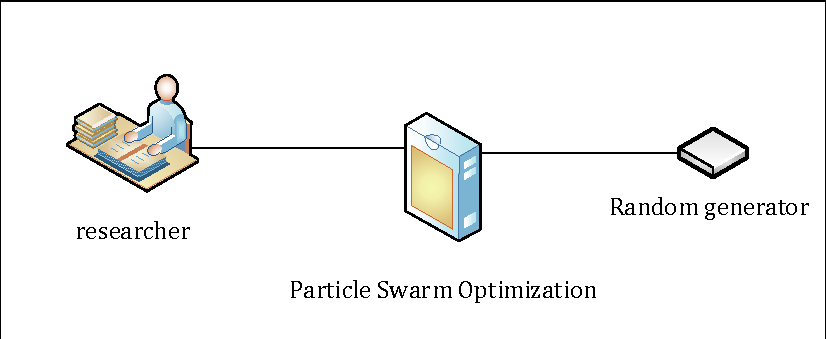
\includegraphics[width=0.7\linewidth]{diagram/description_diagram}
	\caption{Researcher who is using the Particle Swarm Optimization System and a audio source to generate the random element }
	\label{fig:descriptiondiagram}
\end{figure}
\section{Methodology}
Description:

\noindent\fbox{
	\parbox{\textwidth}{
		\textbf{1.} Define a methodology$^1$ using SysML/UML diagrams for the development of your system. Specify SysML/UML diagrams that need to be made in the different phases of the project. Make a short description of each design phases and the SysML/UML diagrams and profiles you decide to use in the methodology. Remember to use references to the papers you have use as inspiration for your work. Decide on an UML$^2$ tool.\cite{Bjerge2017}
	}
}

\section{Requirement specification}
\subsection{Description}

\noindent\fbox{
	\parbox{\textwidth}{
		\textbf{2.} Write a requirement specification with functional and non-functional requirements especially with focus on performance like throughput and latency. The functional requirements can be	described in terms of use cases.
	}
}\citepawesome{Bjerge2017}{1}

%==================== Fully Dressed Use Cases ====================

\subsection{Use Case Beskrivelser - Fully Dressed} \label{sec:usecasebeskrivelser}
For alle Use Cases hvor brugeren navigerer i undermenuer af hovedmenuen, gælder det, at brugeren har mulighed for at gå et skridt tilbage ved at trykke på en ”tilbage knap”. Fremover ved benævningen ”Systemet er operationelt” menes, at systemet er tilsluttet strømforsyning og at alt fungerer samt at systemet er tilsluttet ethernet.

%-------------------- UC1 --------------------
\begin{table}[h]
\begin{tabularx}{\textwidth}{| >{\raggedright\arraybackslash}p{3.3 cm} | >{\raggedright\arraybackslash}X |} \hline

\textbf{Navn:} 						& UC1: Start\\ \hline
\textbf{Mål:}						& At starte systemet helt eller delvist. \\ \hline
\textbf{Initering:}					& Bruger \\ \hline
\textbf{Aktører:} 					& Bruger (primær) \\ \hline
\textbf{Reference:} 					& UC10: Monitorering, UC11: Regulering \\ \hline
\textbf{Antal samtidige forekomster:} & Én \\ \hline
\textbf{Forudsætning:} 				& Systemet er stoppet helt, er operationelt og viser hovedmenuen.\\ \hline
\textbf{Resultat:}					& UC10: Monitorering og evt. UC11: Regulering er startet, systemet viser Hovedmenuen. \\ \hline
\textbf{Hovedscenarie:}				& 

\begin{packed_enum}
\item Bruger trykker på "Monitorering". 
\item System aktiverer UC10: Monitorering. 
\item Bruger trykker på "Regulering". 
	\begin{packed_item}\itemsep1pt \parskip0pt \parsep0pt
	\item {[}Ext 3.a : Bruger trykker ikke "Regulering".{]}
	\end{packed_item}
\item Systemet aktiverer UC11: Regulering.
\item UC1 afsluttes.
\end{packed_enum} \\ \hline
\textbf{Udvidelser:}				&  
\textbf{{[}Ext 3.a : Bruger vælger kun monitorering.{]}}
	\begin{packed_enum}\itemsep1pt \parskip0pt \parsep0pt
	\item Systemet fortsætter ved pkt. 5 i hovedscenariet.
	\end{packed_enum}
\\ \hline
\end{tabularx}
\caption{UC1: Start}
\label{tbl:UC1}
\end{table}


\section{Design Methodology}

\subsection{Description}

\noindent\fbox{
	\parbox{\textwidth}{
		\textbf{3.} Use your design methodology found in \textbf{1}. to describe a SysML/UML model of your system in terms of structure and behavior. Make a suggestion for alternative HW/SW architectures. Decide on which parts of the functionality should be mapped to hardware components and software processes.
	}
}\citepawesome{Bjerge2017}{1}
\section{Design Patterns} \label{designpatterns}

\subsection{Description}

\noindent\fbox{
	\parbox{\textwidth}{
		\textbf{4.} Design the software and apply design patterns that are suitable for your project, and motivate the choice of the used patterns. Use the Two-Part Architecture Model if relevant for the problem. Use the abstract OS package for the ZYBO board.
	}
}\citepawesome{Bjerge2017}{1}\\\\

In the following solution the patterns used are:
\begin{itemize}
	\item State Pattern
	\item Singleton
	\item Command Pattern
\end{itemize}

In this project it has been concluded that the implementation of the State Pattern, Singleton and Command Pattern\citeawesome{RalphJohnsonErichGammaJohnVlissides} profits the project. Each of the patterns are covered in the sections following.

\clearpage

\subsection{GOF State Pattern}\label{dp:state}
The intent of the state pattern is to grant an object the ability to change its behavior when it's internal state changes hence the object will therefore change its class. Consider the state machine diagram in Figure \ref{fig:smdguistate}, page \pageref{fig:smdguistate}, that represents the GUI of the PSOS. The PSOS can be in one of the distinct states: Setup, FindMinima, FindMaxima. \\

When the Zynq CPU starts it enters the Setup state. This receives actions from other classes such as \texttt{ActionUp}, \texttt{ActionDown}, \texttt{ActionNext} and the respond will differ base on the action. For example, the result of an \texttt{StartAction} depends on what the current state is in. In the FindMinima or FindMaxima state the action can occur, the Setup state however does not accept it.\\

As seen in Figure \ref{fig:statemachine}, is the state machine in the project. It was a good choice to use the GOF State Pattern because of the ease to model a state machine and bring it into code. 

\begin{figure}[H]
	\centering
	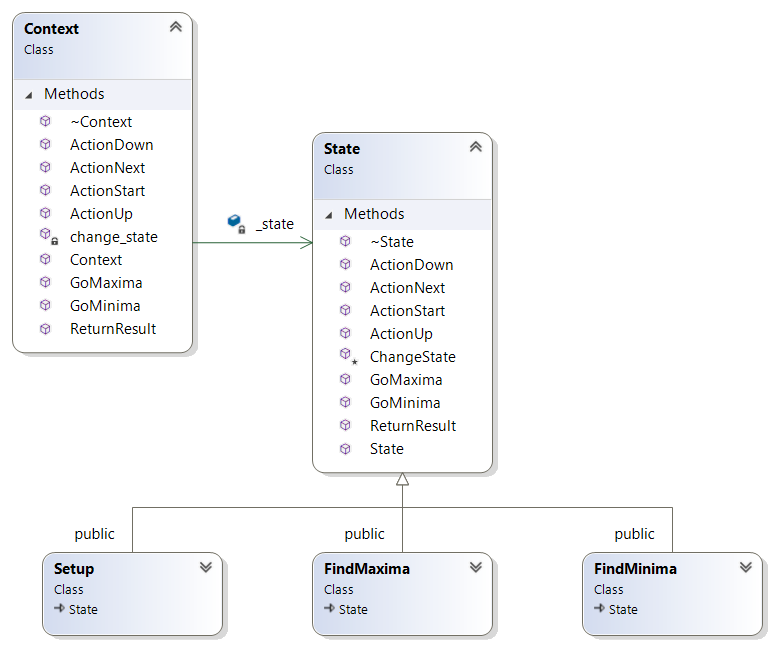
\includegraphics[width=0.8\linewidth]{diagram/StateMachine}
	\caption{An overview of the state machine and it's states.}
	\label{fig:statemachine}
\end{figure}

\clearpage

\subsection{GOF Singleton}\label{dp:singleton}
The intent of the singleton is to guarantee that a class only has one instance therefor providing a single global point of access to it. This is accomplished by making the class itself responsible for keeping track of its instance. The class can guarantee that no other instance can be constructed and therefore it can only have a single way to access the instance.\\

In the project, the GOF Singleton was used to acquire deep history in order for the researcher's variable settings to be kept in the Setup class. It can be seen in the class diagram in Figure \ref{fig:singleton}, where the constructor is private and the only way to get access to the instance of the class, is by using its \texttt{Instance()} method. This guarantees that the acquired instance of the object is always of the same object, unless the destructor have been called.

\begin{figure}[H]
	\centering
	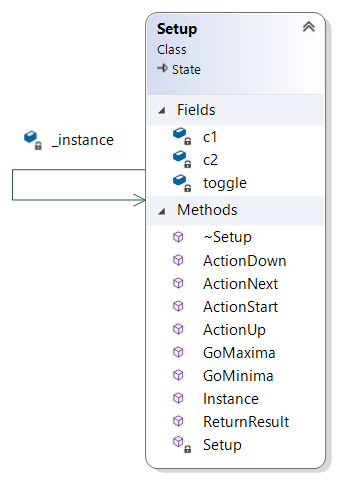
\includegraphics[width=0.35\linewidth]{diagram/singleton}
	\caption[Gof Singleton]{The setup class makes use of the Gof singleton pattern. }
	\label{fig:singleton}
\end{figure}

\clearpage

\subsection{GOF Command Pattern}\label{dp:command}
The intent of GOF Command Pattern is to Encapsulate a request and therefore letting one set different parameters for clients with different requests types. An example could be a message, log requests or other requests. It has support undoable operations (operations that can't be undone ).\\

This allows software engineers to create objects that can interact with the application in a parameterize manner. The command can be stored and moved around like other objects. The main thing about this pattern is the abstract Command class which other commands inherit from. The abstract Command has a interface for executing operations hence an abstract Execute method. Concrete Command subclasses specify a Execute method with the needs for the specific Command. \\
 
In Figure \ref{fig:commands} the commands in the PSOS is shown. The Actions are \texttt{ActionDownCommand}, \texttt{ActionNextCommand}, \texttt{ActionStartCommand} and \texttt{ActionUpCommand}. The Actions are used to change settings in the setup state and start the search for FindMinima and FindMaxima. The transitions commands are \texttt{FindMaximaCommand}, \texttt{ReturnResultCommand} and \texttt{FindMinimaCommand}. By using commands the code handling specific functionality are streamlined and only exist one place, hence it makes it easier to maintain and guards against code duplication.
\begin{figure}[H]
	\centering
	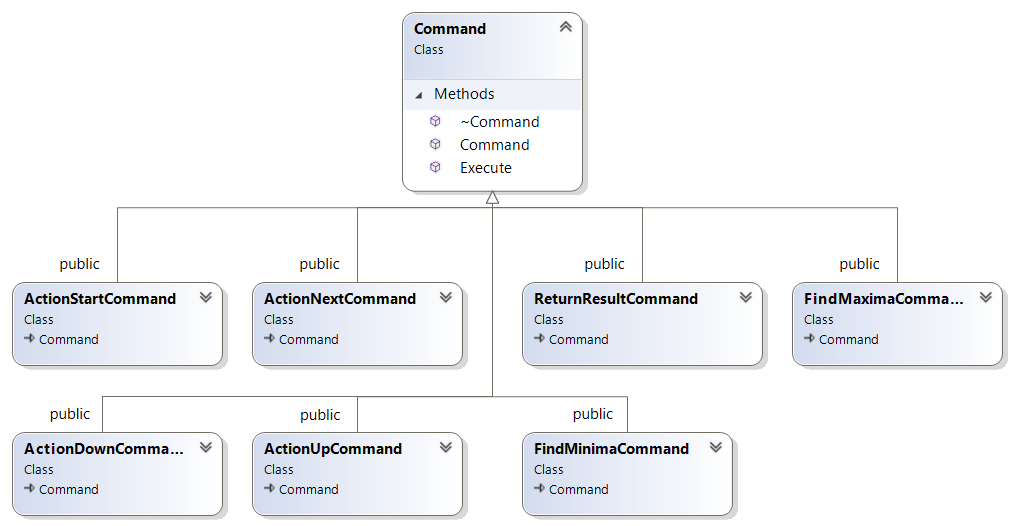
\includegraphics[width=1\linewidth]{diagram/Commands}
	\caption[The commands used to control actions and transitions]{Different Commands in the PSOS. }
	\label{fig:commands}
\end{figure}
\section{Implement and Test}

\subsection{Description}

\noindent\fbox{
	\parbox{\textwidth}{
		\textbf{5.} Select the SysML/UML model for your preferred architecture suggestions in \textbf{3.} Choose a part of the functionality including both hardware and software components to create a model and a testbench in HLS using SystemC or C-code. Simulate and validate your design model. \\\\
		Argue for your choice of modeling language and abstraction level of modeling. Use the reports from the HLS tool to evaluate performance of the design. Assess whether the design is able to fulfill your requirements and constraints.
	}
}\citepawesome{Bjerge2017}{2}
\\\\

% This description is for the implementation itself

\subsection{Description}

\noindent\fbox{
	\parbox{\textwidth}{
		\textbf{6.} Implement and test a part of your system using the ZYBO platform including at least one IP core written and verified with the HLS tool.
	}
}\citepawesome{Bjerge2017}{2}
\section{Conclusion}\label{sc:conclusion}
This project have been conducted in order to analyze if the particle swarm optimization algorithm can be optimized using hardware acceleration. The entire algorithm is implemented in hardware, this could be the reason why so many hardware components are used. A possible way to reduce the hardware requirements would be to only move part(s) of the algorithm onto hardware. Some of parts of particle swarm would be better suited for the Central Processing Unit, such as the generation of random values. But this would also bring trade-offs because of the incensed communication between the hardware and CPU. As for having a random generator in hardware the students didn't know of method to achieve this, though as an afterthought it could properly be implemented by getting random noise from the environment.\\

The math function that was used as the problem to optimize is the peaks function therefore no general functions was used. The peaks function is a rather large, hence hardware requirements would be less if a simpler function was used. Another way to enhance performance would be to have utilized bit wise operations and thereby making the calculations faster.\\

The high level synthesis tools, proved to be very slow, using 2 hours to compile and do synthesis. The code in HLS would need to be optimized to get a more manageable experience. Due to the excessive synthesis time, the choice was made to stop the development of more designs.\\

A key part here was also the use of floating point precision in the search algorithm. As shown in the synthesizer we need quite a many lookup table (LUT), Digital Signal Processor (DSP) and flip-flops. But it is indeed still a design that would possible to run on a bigger FPGA. The ultrascale+ VU37P\citepawesome{XilinxInc.2017}{3} can handle the designs shown in Figure \ref{fig:psossynthesissummary}, but the VU37P was not available in the university lab hence it was not possible to test the real scenario.
%TODO IN BIBLIOGRAPHY - make links clickable, remove escapes in bibTex file
\bibliographystyle{plainnat}
\raggedright
\bibliography{bibtex/collection} \label{ch:bibliography}

\end{document}
